\documentclass[conference]{IEEEtran}
\IEEEoverridecommandlockouts
\usepackage{cite}
\usepackage{amsmath,amssymb}
\usepackage{graphicx}
\usepackage{booktabs}
\usepackage{url}
\usepackage[hidelinks]{hyperref}
\graphicspath{{figs/}}

\begin{document}

\title{Predicting Indoor Location from Wi-Fi Signal Strength:\\
A Phase 1 Baseline on UJIIndoorLoc}

\author{\IEEEauthorblockN{Aviral Mishra, Ved Pawar, Khuswant Rajpurohit,
Prataya Silla, Vansh Jain}
\IEEEauthorblockA{Project 9 --- Applied Machine Learning}}

\maketitle

\begin{abstract}
We estimate where a phone is --- which building, which floor, and its
coordinates --- from the strengths of the Wi-Fi access points it can hear.
Working on the UJIIndoorLoc dataset, we build a deliberately plain baseline:
separate tree models for each target, trained on the dataset's own train/test
split. Random Forest reads the building almost perfectly (99.9\%) and gives the
tightest coordinates (6.96~m median error); XGBoost is the better floor
classifier (92.0\%). Routing each task to whichever model wins it yields a
combined system at 12.0~m mean / 7.1~m median positioning error. Two things
stand out from the error analysis and both carry into Phase~2: a wrong floor
roughly doubles the coordinate error, and accuracy varies by more than a factor
of three across unseen handsets. These numbers set the bar that a shared
multitask network will have to beat.
\end{abstract}

\section{Introduction}
Satellite positioning stops working once you walk indoors, so phones fall back
on whatever signals are around --- and Wi-Fi is everywhere. The idea behind
fingerprinting is simple: record, at many known spots, how loud each nearby
access point sounds, then match a new reading against that map. UJIIndoorLoc is
the standard benchmark for this. It covers three university buildings with
several floors each, and every scan lists the received signal strength (RSSI)
of up to 520 access points.

What makes the problem interesting is that it is really three problems stacked
together. You want the building (a 3-way choice), the floor (5 possibilities),
and a pair of coordinates in metres. These are not independent --- knowing the
building narrows the floors, knowing the floor constrains the coordinates. This
report is Phase~1: a classical machine-learning baseline that treats each of
the three as its own model and measures how far that gets us. It is meant to be
honest and reproducible rather than clever. Phase~2 will replace it with a
network that learns the three targets jointly; the point of a baseline is to
know what ``jointly'' has to improve on.

\section{Data and Exploration}
The training file holds 19{,}937 scans and the separate validation file holds
1{,}111. We use that split as given. Because the validation scans were gathered
later and on different phones, it is a genuine test of generalisation rather
than a reshuffle of the same recordings, and we never fit any transform on it.

Before the first duplicate removal the training set contained 637 scans that
were exact copies of another row --- same signals, same labels --- so we
dropped them and kept 19{,}300 unique scans. The first thing EDA makes obvious
is how little each scan actually sees: the median fingerprint picks up only 17
of the 520 access points (Fig.~\ref{fig:sparsity}), and 96.5\% of the whole
signal matrix is empty. Fifty-five access points are never heard anywhere in
training, so they carry no information and we drop their columns.

\begin{figure}[t]
\centering
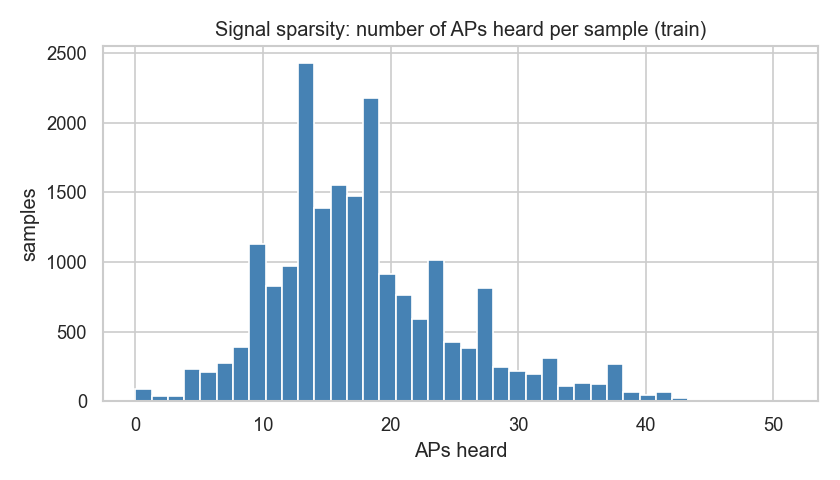
\includegraphics[width=0.85\columnwidth]{eda_aps_per_sample.png}
\caption{How many access points a single scan actually detects. Most scans see
fewer than twenty of the 520 available --- the data is sparse by nature.}
\label{fig:sparsity}
\end{figure}

The three buildings sit in clearly separate places on the map
(Fig.~\ref{fig:layout}), which is a useful hint early on: telling the buildings
apart should be easy, and the real difficulty will be floors and fine
positioning. The floors are not evenly represented. Floor~4 exists only in one
building and shows up in roughly a thousand scans, far fewer than the others,
so we watch it carefully during evaluation.

\begin{figure}[t]
\centering
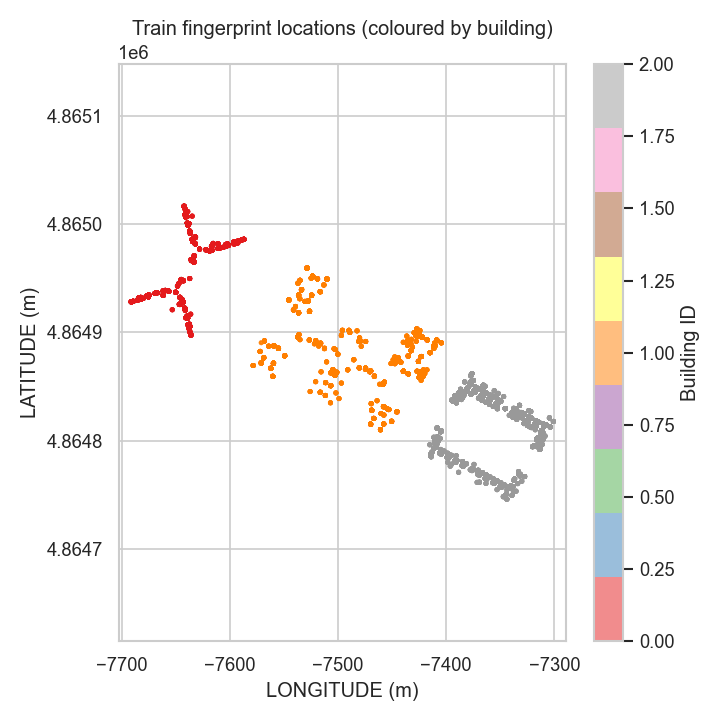
\includegraphics[width=0.82\columnwidth]{eda_spatial_layout.png}
\caption{Training fingerprints plotted at their true coordinates, coloured by
building. The three buildings occupy distinct regions.}
\label{fig:layout}
\end{figure}

\section{Method}
\subsection{Preparing the signals}
UJIIndoorLoc marks an access point that was not heard with the value $+100$,
which is not a real signal level and would wreck any distance or scaling if
left alone. We remap it to $-105$~dBm, just below the weakest genuine reading
($-104$), so ``not heard'' becomes a consistent floor value. The observed RSSI
is then standardised using statistics from the training data only, and the same
transform is applied unchanged to the validation set --- so the validation data
is free to drift rather than being forced to look normalised.

\subsection{Features}
On top of the 465 surviving RSSI columns we add a matching set of 465 binary
``absence'' flags, one per access point, marking whether it was heard. Once the
signals are standardised, a flag is the only thing left that still separates
``weak but heard'' from ``silent,'' and that distinction turns out to matter.
We also compute a handful of per-scan summaries --- how many access points were
heard, the strongest reading and which access point produced it, and the mean,
spread, and range of the heard signals. Altogether the design matrix has 936
columns. Everything here is cheap to compute and easy to explain, which is the
whole idea at this stage.

\subsection{Models}
For each of the three targets we train both a Random Forest and an XGBoost
model: classifiers for building and floor, regressors for the two coordinates
(predicted together). That is six estimators in total, each ignorant of the
others --- which is exactly the gap Phase~2 is meant to close. Hyperparameters
are left at sensible fixed values; we are not tuning a competition entry, we are
drawing a baseline.

\section{Results}
\subsection{Classification and position}
Table~\ref{tab:main} gives the full picture. Building recognition is
effectively solved --- Random Forest misses 1 scan in 1{,}111. Floors are
harder, and the two models split the honours: XGBoost reaches 92.0\% floor
accuracy against Random Forest's 90.7\%, while Random Forest gives noticeably
tighter coordinates (6.96~m median versus 10.06~m). Neither model wins
everything, so the natural thing is to route each task to its stronger model ---
building and coordinates from Random Forest, floor from XGBoost. That combined
system (last row of Table~\ref{tab:main}) gives the best figure on every column
without training anything new: 12.0~m mean and 7.1~m median error, with a 90th
percentile just under 25~m.

\begin{table}[t]
\caption{Validation results. ``Combined'' routes each task to its best model.}
\label{tab:main}
\centering
\small
\begin{tabular}{lcccc}
\toprule
Model & Build.\ & Floor & Coord.\ & Coord.\ \\
      & acc.\   & acc.\ & mean (m) & med.\ (m) \\
\midrule
Random Forest        & 0.999 & 0.907 & 11.66 & 6.96 \\
XGBoost              & 0.997 & 0.920 & 14.52 & 10.06 \\
\textbf{Combined}    & \textbf{0.999} & \textbf{0.920} & \textbf{11.66} & \textbf{6.96} \\
\bottomrule
\end{tabular}
\end{table}

The floor confusion matrix (Fig.~\ref{fig:confusion}) explains where the
remaining floor errors come from: they are almost all off-by-one, a scan placed
on the floor directly above or below its true one. That matches physical
intuition --- a signal bleeds through a ceiling far more easily than through
three of them. The rare Floor~4 is the weakest class, recalled 79.5\% of the
time by XGBoost and only 71.8\% by Random Forest. We tried rebalancing the class
weights to help it and it made things slightly worse, which confirmed the
problem is confusion with the adjacent floor, not simple under-prediction, so we
left the plain model in place.

\begin{figure}[t]
\centering
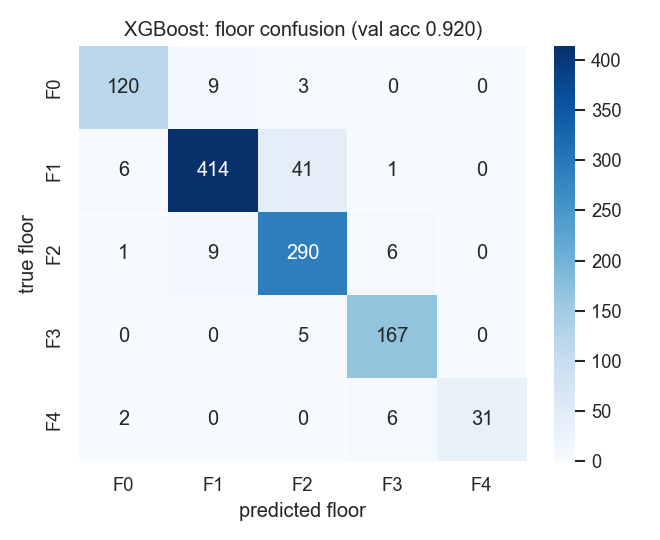
\includegraphics[width=0.8\columnwidth]{confusion_floor_XGBoost.png}
\caption{Floor confusion for XGBoost. Mistakes cluster on the diagonal
neighbours --- almost every error is a single floor up or down.}
\label{fig:confusion}
\end{figure}

\subsection{Where the error lives}
Plotting the coordinate error at each true location (Fig.~\ref{fig:errmap})
shows it is not spread evenly. Corridors with dense fingerprint coverage are
accurate; the large errors sit at building edges and corners where fewer access
points reach. The error CDF (Fig.~\ref{fig:cdf}) makes the model comparison
clean --- Random Forest's curve sits to the left of XGBoost's at every
percentile, so it is not just better on average but better across the whole
distribution of coordinate errors.

\begin{figure}[t]
\centering
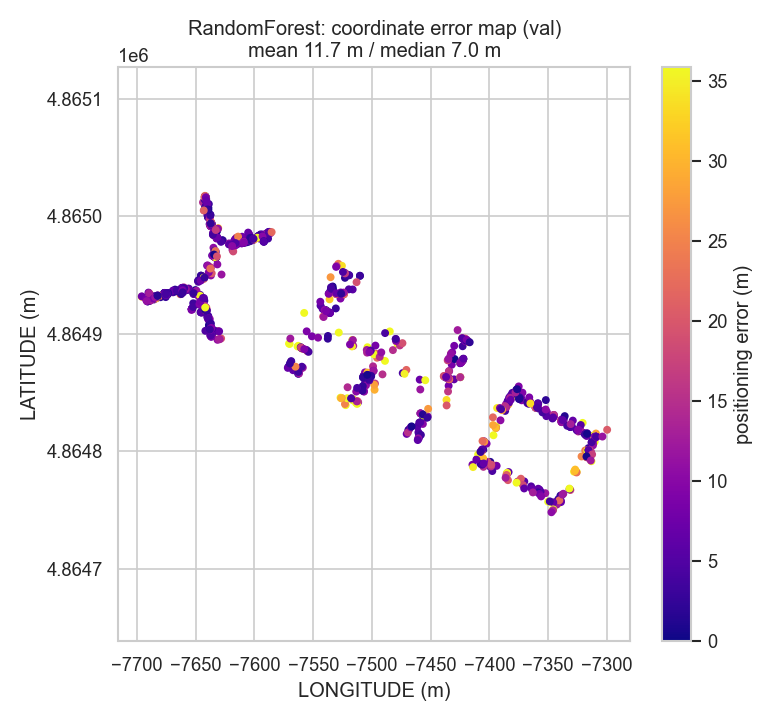
\includegraphics[width=0.82\columnwidth]{error_map_RandomForest.png}
\caption{Coordinate error at each validation point. Error concentrates at
building perimeters where access-point coverage thins out.}
\label{fig:errmap}
\end{figure}

\begin{figure}[t]
\centering
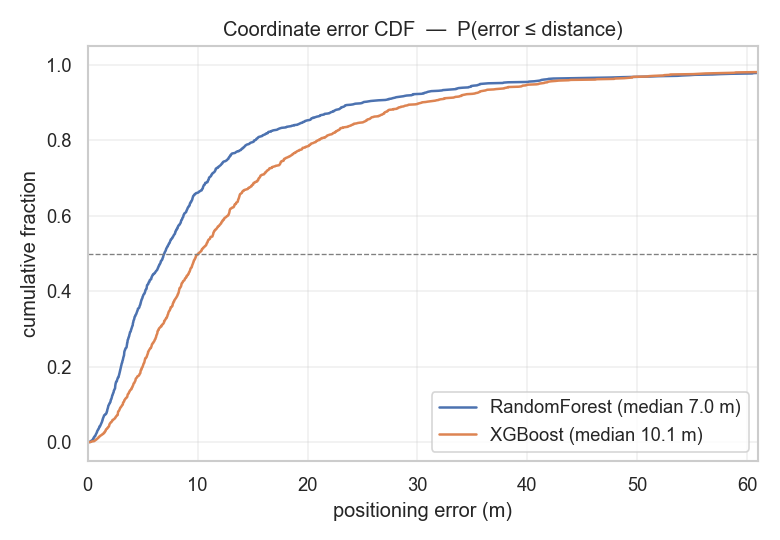
\includegraphics[width=0.85\columnwidth]{error_cdf_comparison.png}
\caption{Cumulative distribution of coordinate error. Random Forest dominates
at every distance.}
\label{fig:cdf}
\end{figure}

One number ties the three tasks together. When the floor is predicted
correctly, the mean coordinate error is 10.2~m; when it is wrong, it jumps to
25.4~m. The targets are coupled --- a classification slip drags the regression
down with it --- and a model that predicted all three at once could in
principle stop that from happening. That is the single clearest argument for
Phase~2.

\subsection{Robustness across devices}
Averages hide a lot. The validation set uses eleven phone models, none of them
seen in training, and the per-phone breakdown (Fig.~\ref{fig:robust}) shows the
error swinging from under 8~m on the best handset to about 31~m on the worst ---
a spread of roughly four to one for Random Forest. One phone in particular is
poor for both models. XGBoost, while less accurate on average, is a little more
even across devices. For a system that would actually ship on many phones, this
device sensitivity is as important as the headline accuracy, and it is not
something a single mean error will ever reveal.

\begin{figure}[t]
\centering
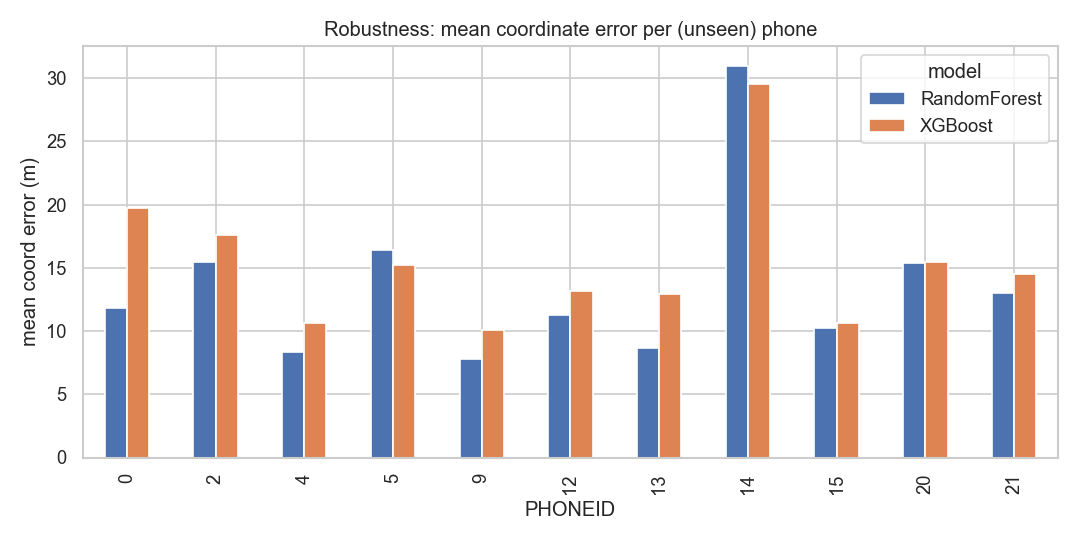
\includegraphics[width=0.9\columnwidth]{robustness_by_phone.png}
\caption{Mean coordinate error per phone model, none seen during training.
Accuracy varies by more than three-fold across handsets.}
\label{fig:robust}
\end{figure}

\section{Discussion and Next Steps}
The baseline does its job: building is essentially solved, floors land in the
low nineties, and median positioning sits around 7~m, all from models that are
easy to reason about and quick to retrain. The honest limits are also clear. We
report on a single supplied split rather than repeated folds, so the figures are
a point estimate, not a confidence interval. We did no hyperparameter search.
And the three models never talk to each other.

That last point is the hand-off to Phase~2. The coupling between floor and
coordinate error, and the uneven behaviour across devices, both suggest that a
shared representation --- one trunk feeding a building head, a floor head and a
coordinate head --- has room to help where separate models cannot. We will keep
the same preprocessing, the same features, and the same split and metrics, so
whatever Phase~2 reports can be compared against this table directly and
fairly.

\section*{Reproducibility}
The pipeline is organised as one script per lifecycle stage (exploration,
preprocessing, features, training, evaluation, visualisation, robustness) and
assembled into a single notebook that reproduces every number and figure here.

\begin{thebibliography}{1}
\bibitem{uji}
J.~Torres-Sospedra \emph{et al.}, ``UJIIndoorLoc: A new multi-building and
multi-floor database for WLAN fingerprint-based indoor localization problems,''
in \emph{Proc.\ IPIN}, 2014.
\bibitem{mtl}
R.~Caruana, ``Multitask learning,'' \emph{Machine Learning}, vol.~28, no.~1,
pp.~41--75, 1997.
\end{thebibliography}

\end{document}
